% Template for Cogsci submission with R Markdown

% Stuff changed from original Markdown PLOS Template
\documentclass[10pt, letterpaper]{article}

\usepackage{cogsci}
\usepackage{pslatex}
\usepackage{float}
\usepackage{caption}

% amsmath package, useful for mathematical formulas
\usepackage{amsmath}

% amssymb package, useful for mathematical symbols
\usepackage{amssymb}

% hyperref package, useful for hyperlinks
\usepackage{hyperref}

% graphicx package, useful for including eps and pdf graphics
% include graphics with the command \includegraphics
\usepackage{graphicx}

% Sweave(-like)
\usepackage{fancyvrb}
\DefineVerbatimEnvironment{Sinput}{Verbatim}{fontshape=sl}
\DefineVerbatimEnvironment{Soutput}{Verbatim}{}
\DefineVerbatimEnvironment{Scode}{Verbatim}{fontshape=sl}
\newenvironment{Schunk}{}{}
\DefineVerbatimEnvironment{Code}{Verbatim}{}
\DefineVerbatimEnvironment{CodeInput}{Verbatim}{fontshape=sl}
\DefineVerbatimEnvironment{CodeOutput}{Verbatim}{}
\newenvironment{CodeChunk}{}{}

% cite package, to clean up citations in the main text. Do not remove.
\usepackage{apacite}

% KM added 1/4/18 to allow control of blind submission


\usepackage{color}

% Use doublespacing - comment out for single spacing
%\usepackage{setspace}
%\doublespacing


% % Text layout
% \topmargin 0.0cm
% \oddsidemargin 0.5cm
% \evensidemargin 0.5cm
% \textwidth 16cm
% \textheight 21cm

\title{Speakers communicate using language-specific information distributions}


\author{Josef Klafka \and Daniel Yurovsky \\
        \texttt{klafka@andrew.cmu.edu} and \texttt{yurovsky@cmu.edu} \\
       Department of Psychology \\ Carnegie Mellon University}

\begin{document}

\maketitle

\begin{abstract}
What role does communicative efficiency play in how we organize our
utterances? In this paper, we present a novel method of examining how
much information speakers in a given language communicate in each word,
surveying numerous diverse languages. We find that speakers produce
frequent and informative words at regular parts of their utterances,
depending on language they use. The information distribution for each
language is derived in part from the features and genealogy of the
language. This robust information distribution characterizes both spoken
and written communication, and emerges in children's earliest
utterances. However, in real-time communication, in-context word
predictability allows listeners to process information at a constant,
optimal rate, regardless of the information distribution in the language
they understand.

\textbf{Keywords:}
information theory; communication; language modeling; computational
modeling
\end{abstract}

\hypertarget{introduction}{%
\section{Introduction}\label{introduction}}

We use language for a variety of purposes like greeting friends, making
records, and signaling group identity. But, these purposes all share a
common goal: Transmitting information that changes the mental state of
the listerner or reader (Austin, 1975). For this reason, language can be
thought of as a code, one that allows speakers to turn their intended
meaning into a message that can be transmitted to a listener or reader,
and subsequently converted by the listener back into an approximation of
the intended meaning (Shannon, 1948). How should we expect this code to
be structured?

If language has evolved to be a code for information transmission, its
structure should reflect this process of optimization (Anderson \&
Milson, 1989). The optimal code would have to work with two competing
pressures: (1) For listeners to easily and successfully decode messages
sent by the speaker, and (2) For speakers to easily code their messages
and transmit them with minimal effort and error. A fundamental
constraint on both of these processes is the linear order of spoken
language--sounds are produced one at a time and each is unavailable
perceptually once it is no longer being produced.

Humans accomodate this linear order constraint through incremental
processing. People process speech continuously as it arrives, predicting
upcoming words and building expectations about the likely meaning of
utterances in real-time rather than at their conclusion (Kutas \&
Federmeier, 2011; Pickering \& Garrod, 2013; Tanenhaus, Spivey-Knowlton,
Eberhard, \& Sedivy, 1995). Since prediction errors can lead to severe
processing costs and difficulty integrating new information on the part
of listeners, speakers should seek to minimize prediction errors.
However, the cost of producing more predictable utterances is using more
words. Thus, the optimal strategy for speakers seeking to minimize their
production costs is to produce utterances that are just at the
prediction capacity of listeners without exceeding this capacity (Aylett
\& Turk, 2004; Genzel \& Charniak, 2002). In other words, speakers
should maintain a constant rate information of as close to the
listener's fastest decoding rate as possible.

This Uniform Information Density hypothesis has found support at a
variety of levels of language from the structure of individual words, to
the syntactic structure of utterances (Jaeger \& Levy, 2007; Piantadosi,
Tily, \& Gibson, 2011; see Gibson et al., 2019 for a review). Further,
speakers make lexical choices that smooth out the information in their
utterances (Jaeger \& Levy, 2007; Mahowald, Fedorenko, Piantadosi, \&
Gibson, 2013). However, while speakers can control which of several
near-synonyms they produce, or whether to produce an optional
complementizer like ``that,'' they cannot control the grammatical
properties of their native language like canonical word order that
impose top-down constraints on the structure of utterances. While
speakers may produce utterances as uniform in information density as
their languages will allow, these top-down constraints may impose
significant variation.

How significant are these top-down constraints? One previous paper
analyzed the information content in English sentences and found a
surprising three-step shape where information first rises, then plateus,
and then sharply rises again at the ends of sentences (Yu, Cong, Liang,
\& Liu, 2016). We build on these ideas, asking (1) Whether this shape
depends on listener's predictive models, (2) Whether this shape varies
across linguistic contexts, and (3) Whether this shape is broadly
characteristic of a diverse set of languages or varies predictably from
language to language. We find that languages are characterized by
highly-reliable but cross-linguisticly variable structures that co-vary
with typological features, but that predictive coding flattens these
shapes across languages, in accord with predictions of the Uniform
Information Density hypothesis.

\hypertarget{study-1-information-in-written-english}{%
\section{Study 1: Information in Written
English}\label{study-1-information-in-written-english}}

\textbf{Describe the Genzel Idea and how to Generalize it to
within-sentence} \textbf{Yu did a thing but it doesn't generalize, we do
it with surprisal} Using their word entropy metric without context, Yu
et al. (2016) found a distinctive three-step distribution for
information in written English sentences in the corpus. The first word
tended to contain little information. While the middle words of
sentences each had more information than the first word, they found a
flat and non-increasing rate of information transmission across the
middle of sentences. The final word contained the most, though not most,
of the information out of any in the sentence, with a noticeable spike
in information. They found the same distribution across sentence
lengths, from sentences with \(15\) words to sentences with \(45\)
words.

\hypertarget{corpus}{%
\subsection{Corpus}\label{corpus}}

Following Yu et al. (2016), we selected the British National Corpus
(BNC) for analysis (British National Corpus Consortium, 2007). The BNC
is a collection of spoken (10\%) and written (90\%) from the turn of the
century, intended to be a representative sample of British English.

\hypertarget{pre-processing}{%
\subsection{Pre-processing}\label{pre-processing}}

We began the XML version of the corpus, and used the
\texttt{justTheWords.xsl} script provided along with the corpus to
produce a text file with one sentence of the corpus on each line.
Compound words (like ``can't'') were combined, and all words were
converted to lowercase before analysis. This produced a corpus of just
over six million utterance of varying lenghts. From these, we excluded
utterances that were too short to allow for reasonable estimation of
information shape (fewer than 5 words), and utterances that were
unusually long (more than 30 words). This exclusion left us with 67.64\%
of the utterances (Fig @ref\{fig:bnc-lengths\}.

\begin{CodeChunk}
\begin{figure}[tb]
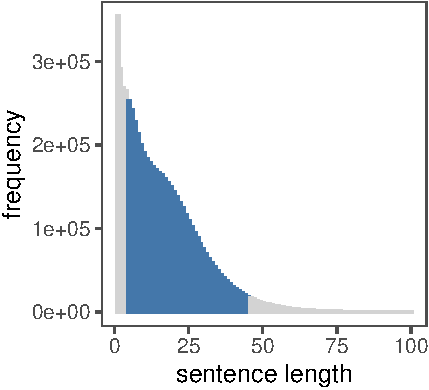
\includegraphics{figs/bnc-lengths-1} \caption[Sentence length distribution in the British National Corpus]{Sentence length distribution in the British National Corpus. Lengths included in analysis are dark.}\label{fig:bnc-lengths}
\end{figure}
\end{CodeChunk}

\hypertarget{estimating-information}{%
\subsection{Estimating information}\label{estimating-information}}

To estimate how information is distributed across utterances, we
computed the lexical surprisal of each word under two different models
(Levy, 2008; Shannon, 1948). Intuitively, the surprisal of a word is a
measure of how unexpected it would be to read that word, and thus how
much information it contains. First, following Yu et al. (2016), we
estimated a unigram model which considers each word independently,
asking how unexpected that word would be in the absence of any context:
\(\text{surprisal}(\text{word}) = -\log P(\text{word})\). This unigram
surprisal measure is a direct transformation of the word's frequency and
thus less frequent words are more surprising.

Second, we estimated a trigram model in which the surprisal of a given
word (\(w_i\)) encodes how unexpected it is to read it after reading the
prior two words (\(w_{i-1}\) and \(w_{i-2}\)):
\(\text{surprisal}(w_{i}) = -log P(w_i|w_{i-1},w_{i-2})\). This metric
encodes the idea that words that are low frequency in isolation (e.g.
``meatballs'') may become much less surprising in certain contexts (e.g.
``spaghetti and meatballs'') but more surprising in others (e.g.
``coffee with meatballs''). In principle, we would like to encode the
surprisal of a word given all of the prior sentential context
(\(\text{surprisal}(w_{i}) = -P(w_i|w_{i-1}w_{i-2}...w_{1})\). However,
the difficulty of correctly estimating these probabilities from a corpus
grow combinatorically with the number of prior words, and in practice
trigram models perform well as an approximation (see e.g. Chen \&
Goodman, 1999; Smith \& Levy, 2013).

\hypertarget{model-details}{%
\subsubsection{Model details}\label{model-details}}

We estimated the surprisal for each word type in the British National
Corpus using the KenLM toolkit (Heafield, Pouzyrevsky, Clark, \& Koehn,
2013). Each utterance was padded with a special start-of-sentence word
``\(\left<s\right>\)'' and end of sentence word ``\(\left</s\right>\)''.
Trigram estimates did not cross sentence boundaries, so for example the
surprisal of the second word in an utterances was estimated as
(\(\text{surprisal}(w_{2}) = -P(w_2|w_{i},\left<s\right>)\).

Naïve trigram models will underestimate the surprisal of words in
low-frequency trigrams (e.g.~if the word ``meatballs'' appears only once
in the corpus following exactly the words ``spaghetti and'', it is
perfectly predictable from its prior two words). To avoid this
underestimation, we used modified Kneser-Ney smoothing which discounts
all ngram frequency counts--reducing the impact of rare ngrams on
probability calculations--and interpolates lower-order ngrams into the
calcuations. These lower-order ngrams are weighted according to the
number of distinct contexts they occur as a continuation (e.g.
``Francisco'' may be a common word in a corpus, but likely only occurs
after ``San'' as in ``San Francisco'', so it receives a lower weighting;
see Chen \& Goodman, 1999).

\hypertarget{averaging-curves}{%
\subsubsection{Averaging curves}\label{averaging-curves}}

To aggregate across utterance lengths, we used dynamic time warping
barycenter averaging (Petitjean, Ketterlin, \& Gançarski, 2011). The
dynamic time warping (DTW) algorithm (Sakoe \& Chiba, 1978) compares
time sequential data, first used for speech recognition to unite
stretched and shifted sound patterns. This algorithm finds a
prototypical time series given variable length series. Something about
length of barycenters. \textbf{Talk about choosing size based on
something about utterance length distribution} \textbf{Maybe we even
want to show this distribution?}

\hypertarget{results}{%
\subsection{Results}\label{results}}

We replicate the Yu et al. (2016) result using the surprisal metric in
place of the entropy metric. We use the frequency-based or
``contextless'' surprisal metric, which determines the average
distribution of information based on word frequencies in a corpus. A
priori we expect that the frequency-based metric will produce a flat
distribution of information across word positions in the BNC. We find
the same frequency-based information trajectory as Yu et al.~with little
information in the first words of utterances and the most information in
the final word, see Figure @ref(fig:bncunigrams).

\begin{CodeChunk}
\begin{figure}[tb]
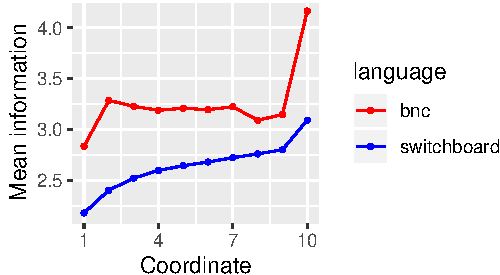
\includegraphics{figs/bncunigrams-1} \caption[BNC and Switchboard frequency-based trigram curves]{BNC and Switchboard frequency-based trigram curves}\label{fig:bncunigrams}
\end{figure}
\end{CodeChunk}

We now include two words of context (trigrams) for each word in our
measurements. We observe a flattening effect of context for both spoken
and written English. After the first word or two, where the listener
does not have access to prior context, then they decode information at a
flat and more or less uniform rate. The contextual information curves
for the BNC and Switchboard are in Figure @ref(fig:bnctrigrams). We also
computed bigram curves with one word of context for each prediction:
these bigram curves resemble the trigram curves.

\hypertarget{experiment-2-english-in-other-contexts}{%
\section{Experiment 2: English in Other
contexts}\label{experiment-2-english-in-other-contexts}}

\textbf{Spoken adult-adult} \textbf{Spoken adult-child} \textbf{Spoken
child}

We now turn to developmental data, and show that frequency-based
information curves characterize child speech from the time a child first
begins speaking as well as adult speech, regardless of utterance length.

We compare this result with spoken English conversations from the
Switchboard telephone conversation corpus (Godfrey, Holliman, \&
McDaniel, 1992). The spoken and written English corpora have the same
information trajectory.

We're going to examine child and child-directed speech from CHILDES
(MacWhinney, 2000) to capture the developmental picture. We use corpora
for Spanish, German, French, Mandarin Chinese and Japanese as well as
English. Mandarin and Japanese are not natively written using the Latin
alphabet, and moreover words are not segmented in their native scripts.
Instead of the native scripts, we use transliterations from the corpus
for each of the Mandarin and Japanese utterances into pinyin for
Mandarin and romanji for Japanese. In these transliterations, words are
previously segmented.

We observe a distinct and characteristic frequency-based information
trajectory for each language, robust across each utterance length. We
see the same distribution of information for both parents and children.
The parent often has more information on average at each word position
in their utterances. This is an effect of the surprisal metric: parents
speak more utterances than their children in most of the corpora, which
inflates the number of tokens they use and increases the surprisal of
hearing a rare word. We include the frequency-based information curve
from the North American English CHILDES collection for comparison. See
Figure~@ref(fig:childesunigrams)

\begin{CodeChunk}
\begin{figure}[tb]
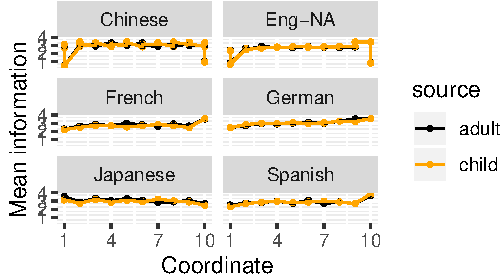
\includegraphics{figs/childesunigrams-1} \caption[CHILDES frequency-based trigram curves]{CHILDES frequency-based trigram curves}\label{fig:childesunigrams}
\end{figure}
\end{CodeChunk}

For the trigram information curves, we see the same contextual smoothing
effect as in English. While the frequency-based information curves may
depend based on the language, the contextual information curves show the
same trajectory cross-linguistically. Using more than two words of
context is difficult for parent-child speech corpora because the
utterances are so short on average (less than \(10\) words). Based on
our results from the CHILDES collections, we hypothesize that the
frequency-based information curves may vary based on the genealogy and
typology of the languages in question. However, this does not extend to
the information curves with two words of context in particular, where
all languages we have seen so far are characterized by the same
information distribution. See Figure @ref(fig:childestrigrams).

\begin{CodeChunk}
\begin{figure}[tb]
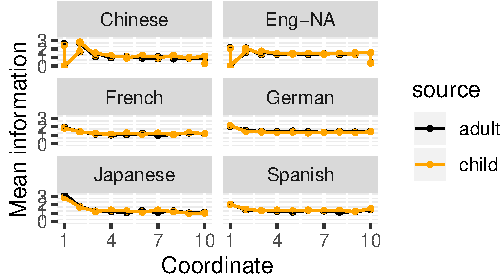
\includegraphics{figs/childestrigrams-1} \caption[CHILDES context-based trigram curves]{CHILDES context-based trigram curves}\label{fig:childestrigrams}
\end{figure}
\end{CodeChunk}

To make a claim about how languages on a larger scale, we need to use
larger corpora and a much larger number of languages.

\hypertarget{experiment-3-large-scale-data-and-linguistic-features}{%
\section{Experiment 3: Large-scale data and linguistic
features}\label{experiment-3-large-scale-data-and-linguistic-features}}

We pulled corpora for \(159\) diverse languages from Wikipedia, each of
which had at least \(10,000\) articles. To compare languages more
rigorously, we used two databases of language similarity features. To
target lexical differences between languages, we used the \(40\)-item
Swadesh list (Swadesh, 1955), retrieved from the ASJP database (Wichmann
et al., 2016). The Swadesh list is a well-known method for comparing
lexical similarity between languages, by quantifying the similarity
between the words on the list for pairs of languages, and is often used
to compare genetic relationships between languages. We computed the
average normalized Levenshtein distance, a string edit distance measure
(LDN; Holman et al., 2008) between each pair of our Wikipedia languages.

As our surprisal metric is a lexical measure, we expect the Levenshtein
distance to be high. To describe more structural relationships, we used
the World Atlas of Language Structures (WALS; Dryer \& Haspelmath, 2013)
to describe the morphology, syntax, phonology, etymology and
semantics--in short the structures in each language. As WALS is a
compiled database from dozens of papers from different authors, most of
the features and languages are fairly sparse. We used a iterative
imputation algorithm for categorical data Multiple Imputation Multiple
Correspondence Analysis (MIMCA; Audigier, Husson, \& Josse, 2017) to
fill in the missing features.

WALS plot goes here

Lexical plot goes here.

What did we learn from this? Unigrams vary kind of with features across
languages. Trigrams are flat all-around.

\hypertarget{conclusion}{%
\section{Conclusion}\label{conclusion}}

In this paper we did model and it showed unique distributions for
unigrams and same distribution for trigrams. Developmental angle.

Follow-up. Possible questions one might have.

\hypertarget{acknowledgements}{%
\section{Acknowledgements}\label{acknowledgements}}

Place acknowledgments (including funding information) in a section at
the end of the paper.

\hypertarget{references}{%
\section{References}\label{references}}

\setlength{\parindent}{-0.1in} 
\setlength{\leftskip}{0.125in}

\noindent

\hypertarget{refs}{}
\leavevmode\hypertarget{ref-anderson1989}{}%
Anderson, J. R., \& Milson, R. (1989). Human memory: An adaptive
perspective. \emph{Psychological Review}, \emph{96}(4), 703.

\leavevmode\hypertarget{ref-audigier2017}{}%
Audigier, V., Husson, F., \& Josse, J. (2017). MIMCA: Multiple
imputation for categorical variables with multiple correspondence
analysis. \emph{Statistics and Computing}, \emph{27}(2), 501--518.

\leavevmode\hypertarget{ref-austin1975}{}%
Austin, J. L. (1975). \emph{How to do things with words}. Oxford
university press.

\leavevmode\hypertarget{ref-aylett2004}{}%
Aylett, M., \& Turk, A. (2004). The smooth signal redundancy hypothesis:
A functional explanation for relationships between redundancy, prosodic
prominence, and duration in spontaneous speech. \emph{Language and
Speech}, \emph{47}(1), 31--56.

\leavevmode\hypertarget{ref-british-national-corpus-consortium2007}{}%
British National Corpus Consortium. (2007). \emph{British national
corpus version 3 (BNC XML edition)}. Oxford: Oxford University Computing
Services. Retrieved from
\href{URL:\%20http://www.natcorp.ox.ac.uk/}{URL: http://www.natcorp.ox.ac.uk/}

\leavevmode\hypertarget{ref-chen1999}{}%
Chen, S. F., \& Goodman, J. (1999). An empirical study of smoothing
techniques for language modeling. \emph{Computer Speech \& Language},
\emph{13}(4), 359--394.

\leavevmode\hypertarget{ref-2013}{}%
Dryer, M. S., \& Haspelmath, M. (Eds.). (2013). \emph{WALS online}.
Leipzig: Max Planck Institute for Evolutionary Anthropology. Retrieved
from \url{https://wals.info/}

\leavevmode\hypertarget{ref-genzel2002}{}%
Genzel, D., \& Charniak, E. (2002). Entropy rate constancy in text. In
\emph{Proceedings of the 40th annual meeting of the association for
computational linguistics} (pp. 199--206).

\leavevmode\hypertarget{ref-gibson2019}{}%
Gibson, E., Futrell, R., Piandadosi, S. T., Dautriche, I., Mahowald, K.,
Bergen, L., \& Levy, R. (2019). How efficiency shapes human language.
\emph{Trends in Cognitive Sciences}.

\leavevmode\hypertarget{ref-godfrey1992}{}%
Godfrey, J. J., Holliman, E. C., \& McDaniel, J. (1992). SWITCHBOARD:
Telephone speech corpus for research and development. In
\emph{{[}Proceedings{]} icassp-92: 1992 ieee international conference on
acoustics, speech, and signal processing} (Vol. 1, pp. 517--520). IEEE.

\leavevmode\hypertarget{ref-heafield2013}{}%
Heafield, K., Pouzyrevsky, I., Clark, J. H., \& Koehn, P. (2013).
Scalable modified kneser-ney language model estimation. In
\emph{Proceedings of the 51st annual meeting of the association for
computational linguistics (volume 2: Short papers)} (pp. 690--696).

\leavevmode\hypertarget{ref-holman2008}{}%
Holman, E. W., Wichmann, S., Brown, C. H., Velupillai, V., Müller, A.,
Bakker, D., \& others. (2008). Advances in automated language
classification. \emph{Quantitative Investigations in Theoretical
Linguistics}, 40--43.

\leavevmode\hypertarget{ref-jaeger2007}{}%
Jaeger, T. F., \& Levy, R. P. (2007). Speakers optimize information
density through syntactic reduction. In \emph{Advances in neural
information processing systems} (pp. 849--856).

\leavevmode\hypertarget{ref-kutas2011}{}%
Kutas, M., \& Federmeier, K. D. (2011). Thirty years and counting:
Finding meaning in the n400 component of the event-related brain
potential (erp). \emph{Annual Review of Psychology}, \emph{62},
621--647.

\leavevmode\hypertarget{ref-levy2008}{}%
Levy, R. (2008). Expectation-based syntactic comprehension.
\emph{Cognition}, \emph{106}(3), 1126--1177.

\leavevmode\hypertarget{ref-macwhinney2000}{}%
MacWhinney, B. (2000). \emph{The childes project: The database} (Vol.
2). Psychology Press.

\leavevmode\hypertarget{ref-mahowald2013}{}%
Mahowald, K., Fedorenko, E., Piantadosi, S. T., \& Gibson, E. (2013).
Info/information theory: Speakers choose shorter words in predictive
contexts. \emph{Cognition}, \emph{126}(2), 313--318.

\leavevmode\hypertarget{ref-petitjean2011}{}%
Petitjean, F., Ketterlin, A., \& Gançarski, P. (2011). A global
averaging method for dynamic time warping, with applications to
clustering. \emph{Pattern Recognition}, \emph{44}(3), 678--693.

\leavevmode\hypertarget{ref-piantadosi2011}{}%
Piantadosi, S. T., Tily, H., \& Gibson, E. (2011). Word lengths are
optimized for efficient communication. \emph{Proceedings of the National
Academy of Sciences}, \emph{108}(9), 3526--3529.

\leavevmode\hypertarget{ref-pickering2013}{}%
Pickering, M. J., \& Garrod, S. (2013). An integrated theory of language
production and comprehension. \emph{Behavioral and Brain Sciences},
\emph{36}(4), 329--347.

\leavevmode\hypertarget{ref-sakoe1978}{}%
Sakoe, H., \& Chiba, S. (1978). Dynamic programming algorithm
optimization for spoken word recognition. \emph{IEEE Transactions on
Acoustics, Speech, and Signal Processing}, \emph{26}(1), 43--49.

\leavevmode\hypertarget{ref-shannon1948}{}%
Shannon, C. E. (1948). A mathematical theory of communication.
\emph{Bell System Technical Journal}, \emph{27}(3), 379--423.

\leavevmode\hypertarget{ref-smith2013}{}%
Smith, N. J., \& Levy, R. (2013). The effect of word predictability on
reading time is logarithmic. \emph{Cognition}, \emph{128}(3), 302--319.

\leavevmode\hypertarget{ref-swadesh1955}{}%
Swadesh, M. (1955). Towards greater accuracy in lexicostatistic dating.
\emph{International Journal of American Linguistics}, \emph{21}(2),
121--137.

\leavevmode\hypertarget{ref-tanenhaus1995}{}%
Tanenhaus, M. K., Spivey-Knowlton, M. J., Eberhard, K. M., \& Sedivy, J.
C. (1995). Integration of visual and linguistic information in spoken
language comprehension. \emph{Science}, \emph{268}(5217), 1632--1634.

\leavevmode\hypertarget{ref-wichmann2016}{}%
Wichmann, S., Müller, A., Wett, A., Velupillai, V., Bischoffberger, J.,
Brown, C. H., \ldots{} others. (2016). The asjp database. \emph{Max
Planck Institute for the Science of Human History, Jena}.

\leavevmode\hypertarget{ref-yu2016}{}%
Yu, S., Cong, J., Liang, J., \& Liu, H. (2016). The distribution of
information content in english sentences. \emph{arXiv Preprint
arXiv:1609.07681}.

\bibliographystyle{apacite}


\end{document}
